\documentclass[aspectratio=169]{beamer}

\usetheme{default}
\usecolortheme{seabird}
\setbeamertemplate{navigation symbols}{}
\setbeamertemplate{footline}[frame number]

\usepackage{amsmath, amssymb}
\usepackage{graphicx}
\usepackage{booktabs}
\usepackage{xcolor}

\graphicspath{{../report/figures/}}

\newcommand{\tbd}[1]{\textcolor{red}{[#1]}}

\title{Modeling Student Priorities}
\subtitle{Workload vs.\ professor quality across the disciplines at Yale}
\author{\tbd{Member A} \and \tbd{Member B} \and Selinam Mortey}
\date{\today}

\begin{document}

% 1 -- A, 0:20
\begin{frame}
  \titlepage
\end{frame}

% 2 -- A, 1:00
\begin{frame}{Why this question}
  \begin{itemize}
    \item Students pick courses on two things they can see in advance: how hard
      it will be, and how good the teaching is.
    \item Nobody knows which one actually drives a course's reputation --- or
      whether that differs across the disciplines.
    \item CourseTable is what students actually read. Is it telling them the
      same thing the raw evaluations say?
  \end{itemize}
  \vfill
  \textbf{Q1.} How much do workload and teaching quality each contribute to a
  course's overall rating, by discipline --- and does CourseTable agree?

  \textbf{Q2.} Which courses are rated far above what the model predicts, and
  where are they?
\end{frame}

% 3 -- B, 1:15
\begin{frame}{Data}
  \begin{columns}[T]
    \begin{column}{0.52\textwidth}
      \textbf{Yale OCE}, Fall 2025
      \begin{itemize}\small
        \item Q4 overall assessment $\;\to\; y$
        \item Q8 workload $\;\to\; x_1$
        \item mean of Q5, Q6 $\;\to\; x_2$
      \end{itemize}
      \vspace{0.5em}
      \textbf{CourseTable}: rating, professor, workload
    \end{column}
    \begin{column}{0.44\textwidth}
      \begin{itemize}\small
        \item 25 courses $\times$ 3 disciplines
        \item random draw, fixed seed
        \item $\geq 8$ responses to be included
        \item blind re-entry QC: \tbd{rate}\%
      \end{itemize}
    \end{column}
  \end{columns}
\end{frame}

% 4 -- C, 1:30
\begin{frame}{Least squares as a projection}
  \begin{columns}[T]
    \begin{column}{0.46\textwidth}
      $A\beta = y$ has no solution: $y$ is not in $\operatorname{Col}(A)$.
      \vspace{0.6em}

      Closest point in the subspace $\Rightarrow$ residual perpendicular to it:
      \[ A^{\mathsf T}e = 0 \]
      \[ A^{\mathsf T}A\,\hat\beta = A^{\mathsf T}y \]
      \[ \hat y = Py,\quad P = A(A^{\mathsf T}A)^{-1}A^{\mathsf T} \]
    \end{column}
    \begin{column}{0.52\textwidth}
      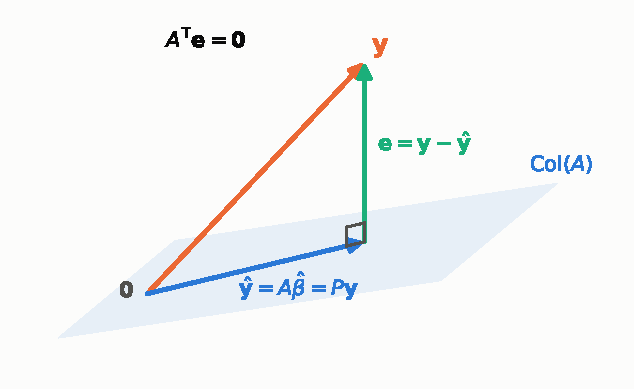
\includegraphics[width=\textwidth]{fig5_projection}
    \end{column}
  \end{columns}
\end{frame}

% 5 -- C, 0:45 (cut to 0:20 if the rehearsal runs long)
\begin{frame}{Checking the answer}
  \begin{itemize}
    \item SVD route: $A = U\Sigma V^{\mathsf T}$, so
      $\hat\beta = V\Sigma^{+}U^{\mathsf T}y$ --- matches.
    \item \texttt{np.linalg.lstsq} and \texttt{statsmodels} OLS --- match.
    \item Orthogonality holds numerically:
      $\max|A^{\mathsf T}e| \approx$ \tbd{1e-15}.
    \item $\kappa(A) \approx$ \tbd{range}; since
      $\kappa(A^{\mathsf T}A) = \kappa(A)^2$, this is the number to watch when
      the predictors are correlated.
  \end{itemize}
\end{frame}

% 6 -- B, 1:30
\begin{frame}{Q1: what carries the rating}
  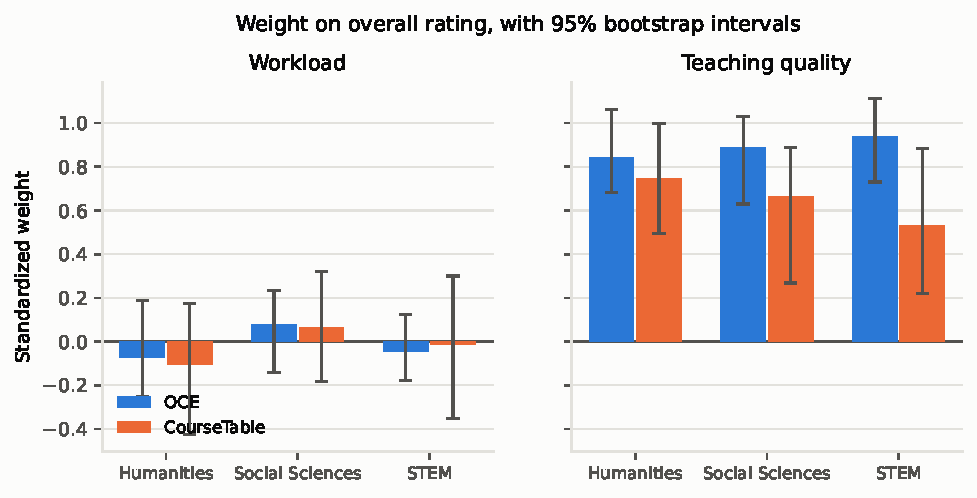
\includegraphics[width=\textwidth]{fig1_weights}
  \vspace{-0.3em}
  \begin{center}\small \tbd{One sentence naming the discipline where workload
  matters most.}\end{center}
\end{frame}

% 7 -- B, 1:00
\begin{frame}{Q1c: does CourseTable say the same thing?}
  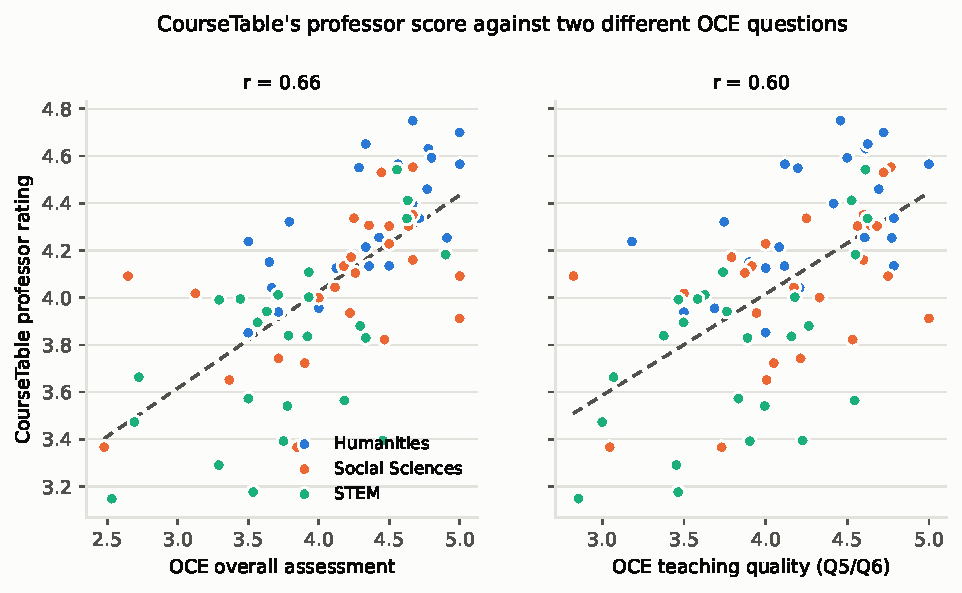
\includegraphics[width=0.92\textwidth]{fig4_circularity}
  \vspace{-0.3em}
  \begin{center}\small \tbd{Does the professor score track the overall question
  more closely than the teaching questions?}\end{center}
\end{frame}

% 8 -- A, 1:15
\begin{frame}{Q2: hidden gems}
  \begin{columns}[T]
    \begin{column}{0.56\textwidth}
      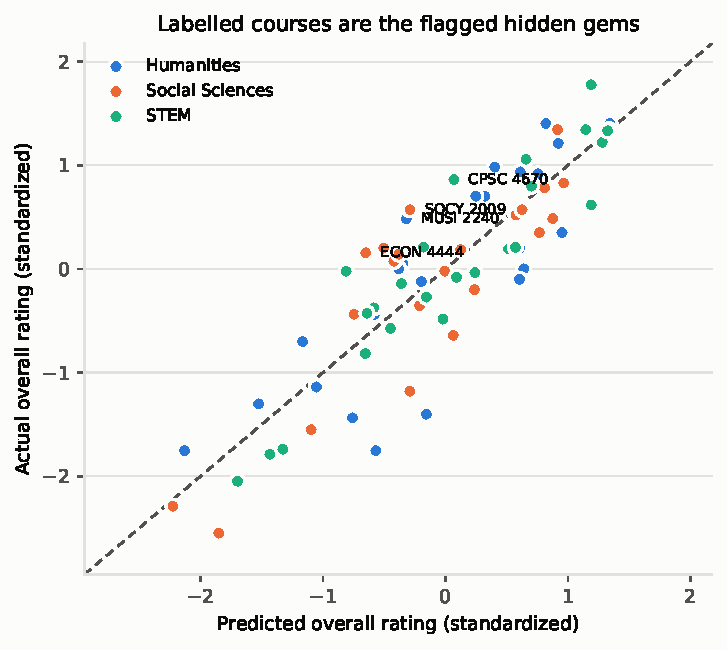
\includegraphics[width=\textwidth]{fig2_actual_vs_predicted}
    \end{column}
    \begin{column}{0.42\textwidth}
      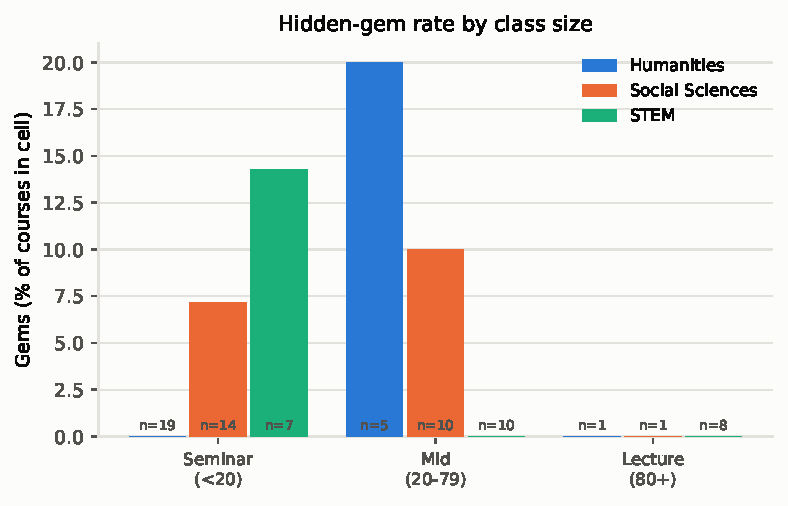
\includegraphics[width=\textwidth]{fig3_gem_rate}
    \end{column}
  \end{columns}
  \begin{center}\small \tbd{Name two gems and where they sit.}\end{center}
\end{frame}

% 9 -- C, 0:45
\begin{frame}{Limitations and conclusion}
  \begin{itemize}
    \item One term; course-level data, so nothing about individual students.
    \item Response bias; ordinal scales treated as numeric; $n = 25$ per
      discipline.
    \item CourseTable's metrics are derived, and we do not control the
      definitions.
  \end{itemize}
  \vfill
  \textbf{Q1.} \tbd{one sentence} \quad \textbf{Q2.} \tbd{one sentence}
\end{frame}

\end{document}
